
\begin{figure}[h]
        \begin{subfigure}[b]{\smallplotsize\textwidth}
                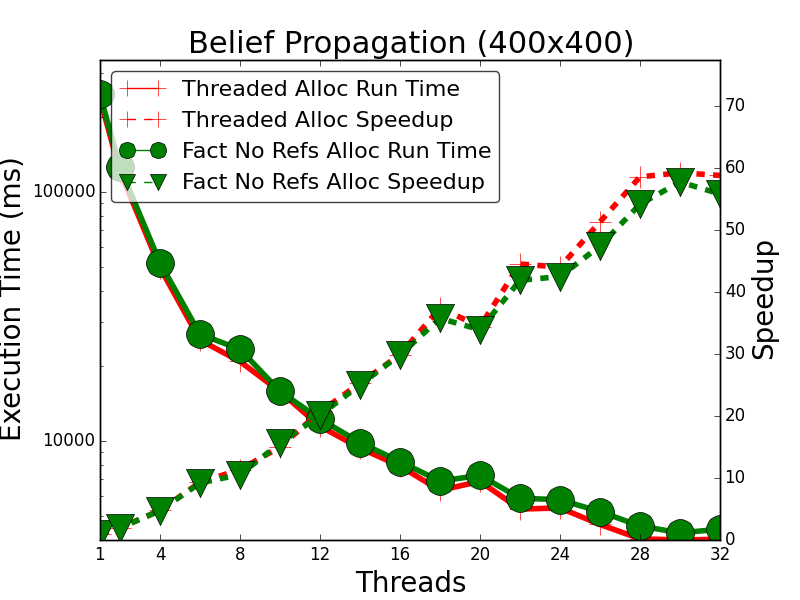
\includegraphics[width=\textwidth]{experiments/scalability/no-refs-allocator-belief-propagation-400.png}
                \label{fig:implementation:no_refs_bp}
        \end{subfigure}
        ~
        \begin{subfigure}[b]{\smallplotsize\textwidth}
                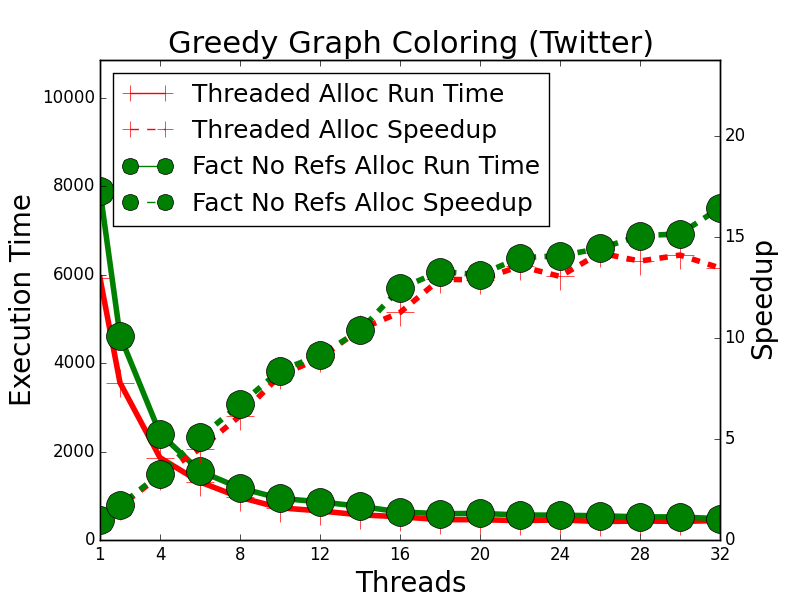
\includegraphics[width=\textwidth]{experiments/scalability/no-refs-allocator-greedy-graph-coloring-twitter.png}
                \label{fig:implementation:no_refs_ggc}
        \end{subfigure}
        ~
        \begin{subfigure}[b]{\smallplotsize\textwidth}
                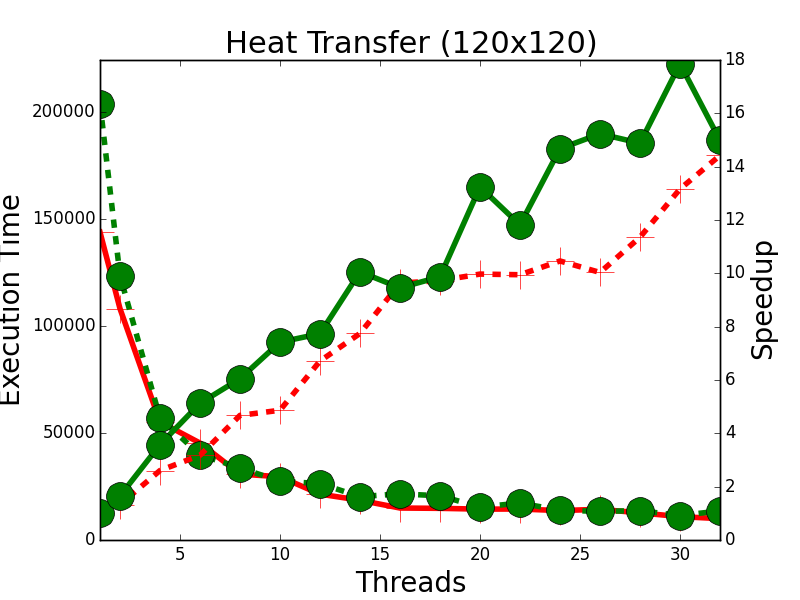
\includegraphics[width=\textwidth]{experiments/scalability/no-refs-allocator-new-heat-transfer-120.png}
                \label{fig:implementation:no_refs_ht}
        \end{subfigure}
        ~
        \begin{subfigure}[b]{\smallplotsize\textwidth}
                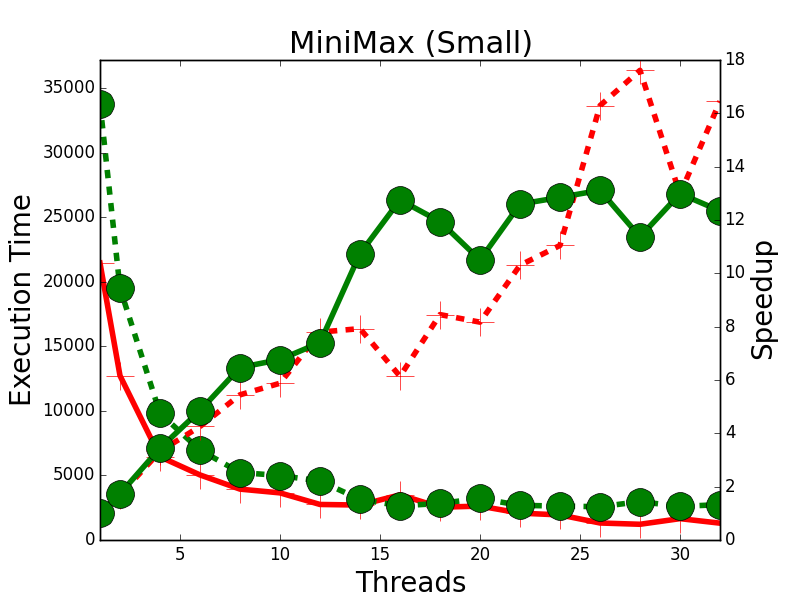
\includegraphics[width=\textwidth]{experiments/scalability/no-refs-allocator-min-max-tictactoe-small.png}
                \label{fig:implementation:no_refs_minimax}
        \end{subfigure}
        ~
        \begin{subfigure}[b]{\smallplotsize\textwidth}
                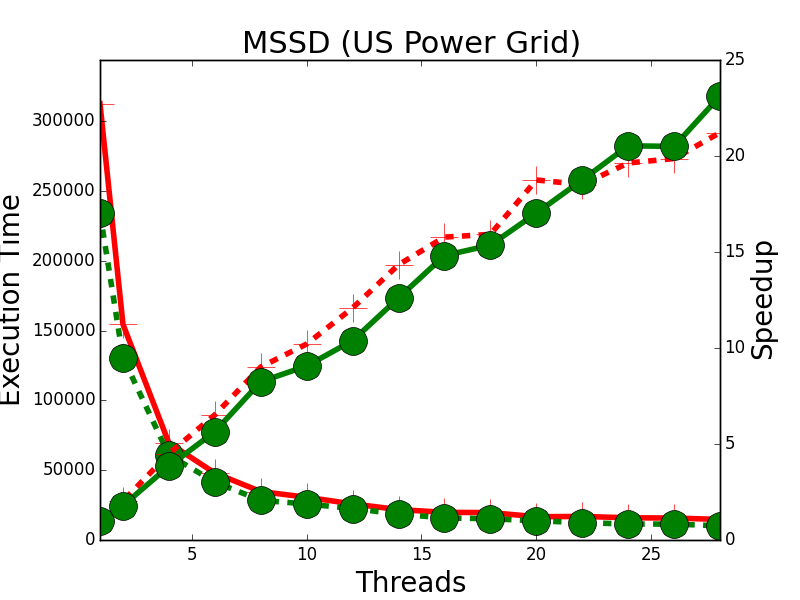
\includegraphics[width=\textwidth]{experiments/scalability/no-refs-allocator-shortest-uspowergrid.png}
                \label{fig:implementation:no_refs_sssp}
        \end{subfigure}
        ~
        \begin{subfigure}[b]{\smallplotsize\textwidth}
                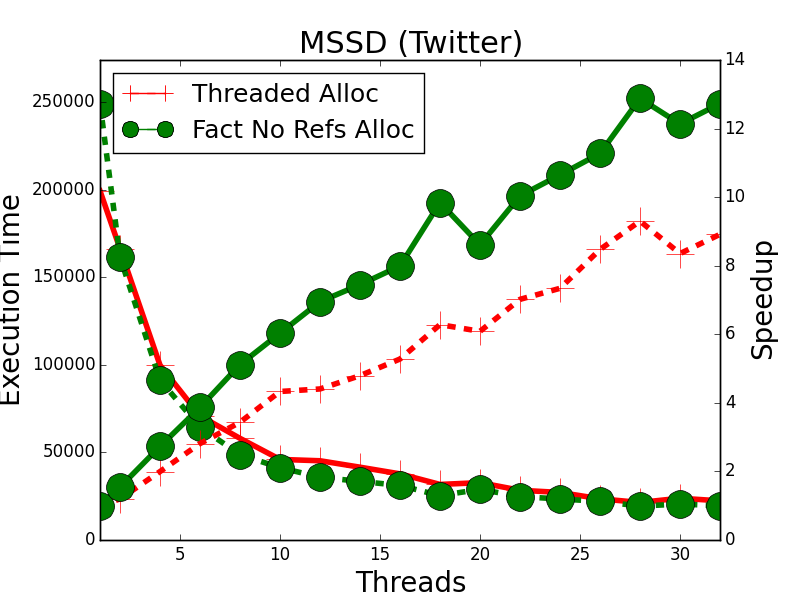
\includegraphics[width=\textwidth]{experiments/scalability/no-refs-allocator-shortest-twitter.png}
                \label{fig:implementation:no_refs_sssp}
        \end{subfigure}\\
        \begin{subfigure}[b]{\smallplotsize\textwidth}
                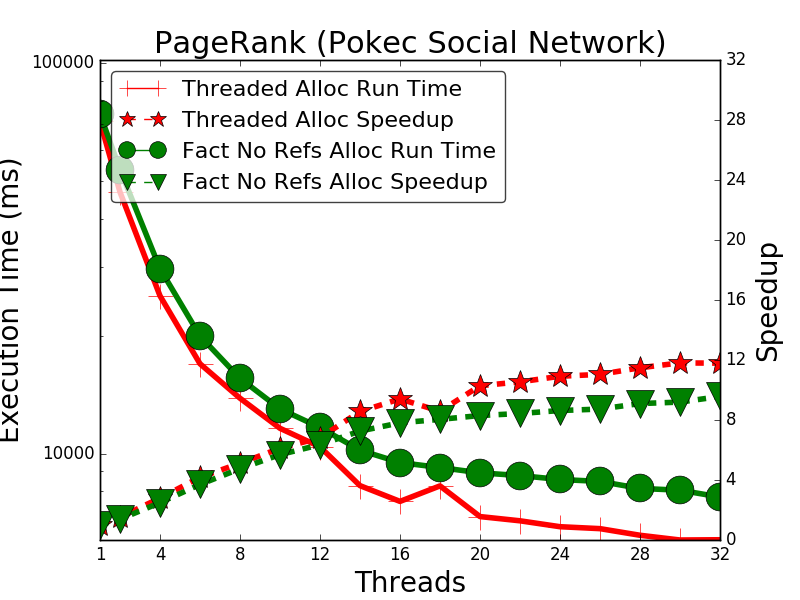
\includegraphics[width=\textwidth]{experiments/scalability/no-refs-allocator-pagerank-pokec.png}
                \label{fig:implementation:no_refs_pagerank}
        \end{subfigure}
        ~
        \begin{subfigure}[b]{\smallplotsize\textwidth}
                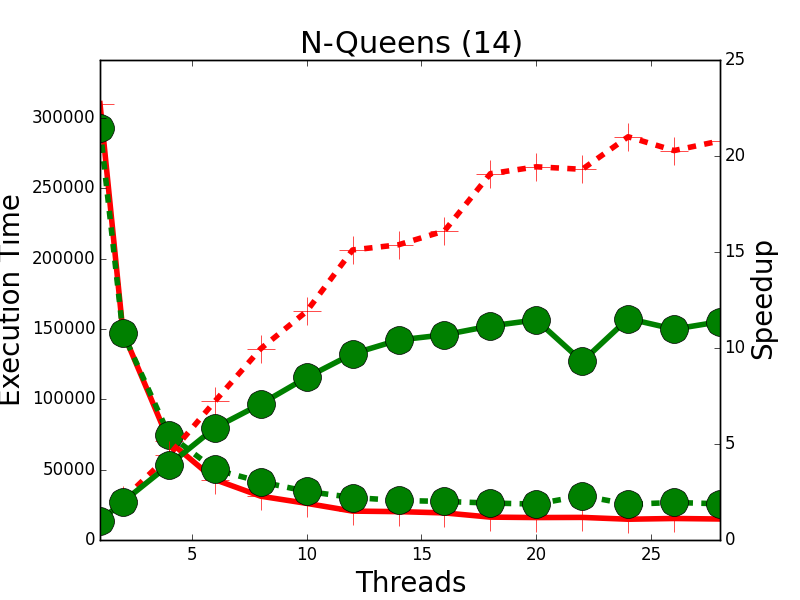
\includegraphics[width=\textwidth]{experiments/scalability/no-refs-allocator-8queens-14.png}
                \label{fig:implementation:no_refs_queens}
        \end{subfigure} \\

        \mycap{Comparing the threaded allocator described in
           Section~\ref{section:implementation:allocation} against the fact
           allocator without reference counting. The threaded allocator is
           represented by plus markers, while the fact allocator is represented
           by circular markers. Note that the two speedup lines (right axis) use
        dashed lines, while the two lines representing the run time (left axis)
     are contiguous.}

        \label{fig:implementation:no_refs_results}
\end{figure}
